\documentclass{sysuthesis}

%%
% 论文相关信息
% 本文档中前缀"c-"代表中文版字段, 前缀"e-"代表英文版字段
% modifyer: 黄俊杰(huangjj27, 349373001dc@gmail.com)
% update date: 2017-04-13
%%

% 标题
% 论文题目应以简短、明确的词语恰当概括整个论文的核心内容,避免使用不常见的缩略词、缩写字。读者通过标题可大致了解毕业设计(论文)的内容、专业的特点和科学的范畴。中文题目一般不宜超过 24 个字,必要时可增加副标题。外文题目一般不宜超过 12 个实词

% 封面标题。由于技术所限,封面题目过长的划分交由用户您进行定夺
% 这也能让您的论文封面看起来更有美感
\covertitlefirst{通用斑马线检测与识别}
\covertitlesecond{}

% Author:   Souler Ou
% 修改者:    欧一锋
% Date:     3/30/2018
% Mail:     ou@souler.cc
%如果英文标题过长可以使用此两项作为表三(答辩记录表)的标题。
\etitlefirst{A Robust Method For Zebra Crossing Detection}
\etitlesecond{}

% 另外一种封面的论文题目. 换行使用换行符("\\")
%\title{
%    中山大学 \\
%    本科毕业论文非正式模版
%}

% 中文标题
\ctitle{通用斑马线检测与识别}
\etitle{A Robust Method For Zebra Crossing Detection}

% 解决英文摘要页标题过长问题 (Issue 49&63)
% 当\etitle的长度超过页边距时,请使用下面的命令自行断行
% 此操作只影响英文摘要页的标题,不影响页眉的标题
% 如果不需要断行,将\eabstracttitlesecond{ }留空即可
\eabstracttitlefirst{A Robust Method For Zebra Crossing Detection} 
\eabstracttitlesecond{}

% 作者详细信息
\author{王天宇}
\cauthor{王\ 天\ 宇}    % 封面作者
\eauthor{Tianyu Wang}
\studentid{14331265}
\cschool{数据科学与计算机学院}

\cmajor{软件工程}
\emajor{Software Engineer}

% 指导老师
\cmentor{胡继华}
\ementor{Jihua Hu}

     % 论文相关信息
%%
% 开题报告
% modifier: 黄俊杰(huangjj27, 349373001dc@gmail.com)
% update date: 2017-05-14

% 选题目的
\objective{

}

% 思路
\methodology{

}

% 研究方法/程序/步骤
\researchProcedure{

}

% 相关支持条件
\supportment{

}

% 进度安排
\schedule{

}

% 指导老师意见
\proposalInstructions{

}

   % 开题报告内容
%%
% 摘要信息
% 本文档中前缀"c-"代表中文版字段, 前缀"e-"代表英文版字段
% 摘要内容应概括地反映出本论文的主要内容,主要说明本论文的研究目的、内容、方法、成果和结论。要突出本论文的创造性成果或新见解,不要与引言相 混淆。语言力求精练、准确,以 300—500 字为宜。
% 在摘要的下方另起一行,注明本文的关键词(3—5 个)。关键词是供检索用的主题词条,应采用能覆盖论文主要内容的通用技术词条(参照相应的技术术语 标准)。按词条的外延层次排列(外延大的排在前面)。摘要与关键词应在同一页。
% modifier: 黄俊杰(huangjj27, 349373001dc@gmail.com)
% update date: 2017-04-15
%%

\cabstract{
本文的研究目的是设计一个能够检测道路中的斑马线的方法,对于检测方法的额外要求是具有通用性和鲁棒性,即对于拍摄条件、拍摄器材和拍摄角度没有要求,对于图片分辨率不高、天气变化、地面湿润等条件不敏感。研究内容首先由已有的双极系数法引入,通过兴趣区域生成的方法改善双极系数法的计算量。该方法取自RCNN算法当中,是本文的核心进展之一。通过分析双极系数法的局限性,进一步挖掘图像中双极系数无法捕捉到的特性,提出基于直线提取算法和字符匹配算法的新判据,这一判据改善了前人只通过直线提取的个数判断的缺陷,大幅提高了识别准确率。在统计特征和形态特征之外,尝试利用纹理特征提取技术结合机器学习算法进一步降低了算法的误识率。综上所述,本文通过改进已有方法,和引入新方法,在斑马线识别问题上,识别率和鲁棒性上均有提高,最后达到了约90\%的识别准确率。
}
% 中文关键词(每个关键词之间用“;”分开,最后一个关键词不打标点符号。)
\ckeywords{图像处理;特征提取;斑马线识别;双极系数}

\eabstract{
The purpose of this paper is to design a method that can detect zebra crossings in roads. The additional requirements for this detection methods are versatility and robustness such that there are no limits for shooting conditions, shooting equipments and shooting angles, low quality of photos, weather changes, wet ground and other conditions have little influence to the detection process. The research begins with the existing bipolar coefficient method, and then optimizing the complexity of the bipolar coefficient method by generation of region of interest. This method is taken from the RCNN algorithm and is one of the core progress of this paper. By analyzing the limitations of the bipolar coefficient method, the characteristics of the bipolar coefficients that can not be captured in the image are further excavated, and a new criterion based on the line extraction algorithm and the string matching algorithm is proposed. This criterion improves the predecessors' method which only considered the number of lines. The change significantly improved the recognition accuracy. In addition to statistical and morphological features, the techniques using texture feature extraction combined with machine learning algorithms has further reduced the false positive rate of the algorithm. In summary, by improving the existing methods and introducing new methods, this paper improves the recognition rate and robustness on the zebra crossing recognition problem, and finally reaches about 90\% of the recognition accuracy rate.
}
% 英文文关键词(每个关键词之间用半角加空格分开, 最后一个关键词不打标点符号。)
\ekeywords{image processing;feature extraction;zebra-crossing detection;bipolarity}

     % 摘要内容
%%
% 成绩评定记录表
% modifier: 黄俊杰(huangjj27, 349373001dc@gmail.com)
% update date: 2017-05-17

\gradingComment{
  某某同学针对什么问题研究了什么算法/实现了什么系统/针对这个系统做了什么测试,本文选题合理,实验结果表明技术路线……论文写作规范,引用文献充分,符合中山大学本科论文的规范,是篇优秀/良好/中等/合格的论文。
}
    % 成绩评定记录表评语
%%
% 四次进度报告相关信息

% Author:   Souler Ou
% 修改者:    欧一锋
% Date:     3/30/2018
% Mail:     ou@souler.cc

% 第一次进度报告
\firstsummary{
	\begin{adjustwidth}{2em}{2em}
		在这一阶段,XXX工作基本完成,主要在如下几个方面:
		\begin{enumerate}
			\item 完成了第一项。
			\item 完成了第二项
			\item 完成了第三项。 
		\end{enumerate}
	\end{adjustwidth}
}
% 第2次进度报告
\secondsummary{
	\begin{adjustwidth}{2em}{2em}
		...
	\end{adjustwidth}
}
% 第3次进度报告
\thirdsummary{
	\begin{adjustwidth}{2em}{2em}
		...
	\end{adjustwidth}
}
% 第4次进度报告
\fourthsummary{
	\begin{adjustwidth}{2em}{2em}
		...
	\end{adjustwidth}
}
% 第1次老师评价
\firstcomment{
	\begin{adjustwidth}{2em}{2em}
		论文完成情况良好。
	\end{adjustwidth}
}
% 第2次老师评价
\secondcomment{
	\begin{adjustwidth}{2em}{2em}
		...
	\end{adjustwidth}
}
% 第3次老师评价
\thirdcomment{
	\begin{adjustwidth}{2em}{2em}
		...
	\end{adjustwidth}
}
% 第4次老师评价
\fourthcomment{
	\begin{adjustwidth}{2em}{2em}
		...
	\end{adjustwidth}
}
% 老师总评价
\finalcomment{
	\begin{adjustwidth}{2em}{2em}
		...
	\end{adjustwidth}
}   % 过程检查报告数据
\begin{document}
    % 论文前置部分
    \frontmatter
        \pagenumbering{Roman}
        \maketitle    % 封面
        \makeProposal% 开题报告
        \makeProgressCheck  % 过程检查记录表
        \makeDefenseRecord  % 答辩情况等级表
        \makedisclaim       % 学术诚信声明
        \makeabstract       % 中英文摘要
        \maketableofcontents        % 目录
        \makelistoffiguretable

    % 论文主体部分
    \mainmatter
        % 引言

        % 正文
        %%
% 引言或背景
% 引言是论文正文的开端,应包括毕业论文选题的背景、目的和意义;对国内外研究现状和相关领域中已有的研究成果的简要评述;介绍本项研究工作研究设想、研究方法或实验设计、理论依据或实验基础;涉及范围和预期结果等。要求言简意赅,注意不要与摘要雷同或成为摘要的注解。
% modifier: 黄俊杰(huangjj27, 349373001dc@gmail.com)
% update date: 2017-04-15
%%

\chapter{引言}
%定义,过去的研究和现在的研究,意义,与图像分割的不同,going deeper
\label{cha:introduction}
\section{选题背景与意义}
\label{sec:background}
% What is the problem
% why is it interesting and important
% Why is it hards, why do naive approaches fails
% why hasn't it been solved before
% what are the key components of my approach and results, also include any specific limitations,do not repeat the abstract
%contribution

通用斑马线检测,意在提出对于分辨率,拍摄角度,光照条件,画面占比没有特殊苛刻要求的斑马线检测和识别算法。问题的关键有两部分,一是如何精准检出斑马线,二是如何提高系统的鲁棒性,降低识别系统对于附加条件的要求。由于自动驾驶技术的兴起和导盲系统的完善,对于交通标志识别的需求日益迫切。斑马线是行车路口和人车交汇点的重要标志,在自动驾驶的行车区域划定和盲人的行走辅助当中都有重要作用。目前与交通标志识别有关的领域分别使用了一些领域相关的斑马线识别技术:例如遥感领域、自动驾驶领域、盲人辅助领域,各种技术都有各自的长处和局限,通过提供一个通用的高准确率低误识率的斑马线的检测与定位技术,可以为这些领域提供极大的便利。斑马线的视觉特征非常明显,但是其检测算法并不直观,简单的算法往往会陷入窘境,例如道路标志褪色造成的“白线”变“灰线”,或者会被一只黑白相间的猫所迷惑。本题提出的算法,在基本保证实时性的同时,能够利用多种判据规避相似图形,同时对于视角等条件没有要求。


\section{国内外研究现状和相关工作}
\label{sec:related_work}
京都工业大学的Mohammad Shorif Uddin和Tadayoshi Shioyama在2005年提出将双极系数法\cite{bipolar}应用于盲人辅助行走系统中识别斑马线,双极系数法运算量小结果比较准确受到广泛传播,二人之后再次提出基于IPM变换的改进方法。2013年北方工业大学的王一丁和徐超改良了检测流程中的IPM变换\cite{ipm}。在2015年,武汉大学测绘学院的阎利和黄亮将双极系数法应用于高空球形摄像机中,并且结合了Hough变换来提取直线。为了黄新和林倩,在2017年进一步提出了双极系数和直线提取的一些改进方法。斑马线识别实际是物体识别的一个特例,因此本文也涉及物体识别和图像分割的通用方法,例如Pedro F. Felzenszwalb和Daniel P. Huttenlocher提出的基于图论的图像分割算法\cite{segmentation},被广泛应用来实现Selective Search,产生深远影响。

\section{本文的论文结构与章节安排}

\label{sec:arrangement}
本文共分为五章,各章节内容安排如下:

第一章引言。

第二章图像特征提取,本章介绍传统图像处理方法在斑马线识别这个具体问题上的应用技术,比较多种方法的优势和劣势,详细介绍和讨论双极系数法和灰度共生矩阵及其特征值。

第三章兴趣区域生成,本章重点介绍一种高效的图像分割算法,以及图像分割在斑马线识别问题中减少计算量和提高准确性等重要意义。

第四章检测与识别算法,本章从双极系数、Hough变换到纹理提取,完整的串联出斑马线检测的程序,并给出详细的中间过程说明。

第五章试验结果,本章包括本文介绍的多种方法在测试集上的准确率和误识率数据,和典型已知错误的分析。

第六章总结与展望,是本文的最后一章,是对本文内容的整体性总结以及对未来工作的展望。


        \newclearpage
        \chapter{图像特征提取}
\label{cha:feature}

\section{双极系数}
\label{sec:bipolar}
双极系数法最早由京都工业大学的Mohammad Shorif Uddin和Tadayoshi Shioyama提出,作为一种鲁棒的斑马线检测算法,替代实时性和准确性不足的“消逝点法”。它的鲁棒性表现在不受多种光照条件和气候变化的影响。但该特征受道路磨损的影响较大。 \par
它的算法描述如下:对于一副图像,将它的灰度分布记为$p_0(x)$。将灰度像素分为低灰度区域和高灰度区域,那么$p_0(x)$可以表示为
\begin{align}
	p_0(x)=\alpha p_1(x) + (1-\alpha)p_2(x)
\end{align}
其中$p_1(x)$表示低灰度的分布,$p_2(x)$表示高灰度的分布。以上变量的均值和方差可以表示为
\begin{align}
	\mu_i=\int_{-\infty}^{+\infty}xp_i(x)dx, (i = 1, 2, 3) \\
	\sigma_i^2=\int_{-\infty}^{+\infty}(x-\mu_i)^2p_i(x)dx, (i = 1, 2, 3)
\end{align}
综合以上三式,
\begin{align}
	\sigma_0^2=\alpha \sigma_1^2+(1-\alpha)\sigma_2^2+\alpha(1-\alpha)(\mu_1-\mu_2)^2
\end{align}
观察(2.4)可以发现,灰度分布的总体方差可以表示为两部分方差和均值差平方的加权和,那么当总体方差主要受均值差影响时,我们认为图像是完全双极性的,既$\sigma_0^2\approx \alpha(1-\alpha)(\mu_1-\mu_2)^2$。所以定义双极性的函数为:
\begin{align}
	\gamma \equiv \frac{1}{\sigma_0^2} \alpha(1-\alpha)(\mu_1-\mu_2)^2 
\end{align}\par
式(2.5)告诉我们,$0 \leq \gamma \leq 1$,并且当$\gamma=1$时,说明低灰度分布和高灰度分布的内部方差均为0,此时图像具有完全的双极性。当$\gamma=0$时,低灰度分布和高灰度分布均值相同或某一个灰度区域不存在,既图像完全没有双极性。

\section{灰度共生矩阵和特征值}
\label{sec:cogrey}
斑马线有黑白相间,间隔相同的特线,因此可以看做一种纹理,通过灰度共生矩阵(GLCM,Gray-Level Co-occurrence Matrix)将纹理信息提取出来。纹理是由灰度分布在空间域上反复出现而形成的,因此图像中相隔某个角度某个距离的像素的灰度之间有相关性。共生矩阵是指给定偏移量后共现灰度值的分布。它有如下特点:
\begin{enumerate}
	\item 偏移量是指,$(\Delta x, \Delta y)$或者$(\Delta \rho, \Delta \theta)$,$x$和$y$分别表示偏移的横纵坐标,$\rho$和$\theta$分别表示偏移的圆心距和极角
	\item 一个灰度定义域为$[0,p]$的图像的灰度共生矩阵是一个$p \times p$的矩阵
	\item 灰度共生矩阵中坐标为$(x, y)$的位置的值是$x$和$y$这两个灰度在给定偏移量下共同出现的次数
\end{enumerate}\par
对于一个矩阵A来说,它的灰度共生矩阵C可以表示为
\begin{align}
C_{\Delta x, \Delta y}(i,j)=\sum_{x=1}^n\sum_{y=1}^m\begin{cases} 1, & \text{if }A_{i,j}\text{ and }A_{x+\Delta x, y+\Delta y}=j \\ 0, & \text{otherwise}\end{cases}, (offset \equiv (\Delta x, \Delta y))
\end{align}
然而求出的灰度共生矩阵维数很大,无法很直观的使用,因此介绍与本题相关的灰度共生矩阵的特征值:熵(entropy),能量(energy),相关性(correlation),对比度(contrast)。
\subsection{熵}
\begin{align}
ENT=\sum_{i,j\in A} -log(p_{i,j})p_{i,j}
\end{align}\par
把信息中排除了冗余后的平均信息量是信息熵,灰度共生矩阵的信息熵反映了图像邻域内的信息熵大小,越复杂的纹理所计算出的熵越大,反之较小。斑马线的特征是其灰度共生矩阵的熵较小。
\subsection{能量}
\begin{align}
ASM=\sum_{i,j\in A} p_{i,j}^2
\end{align}\par
能量是反映图像灰度分布均匀和纹理粗细的重要指标,当纹理较细致纹理问分布均匀时,灰度共生矩阵的能量较大,反之较小。斑马线体现出的特征是其灰度共生矩阵的能量不能过大也不能过小。可以观察到,灰度全为最低灰度时是灰度共生矩阵的能量的下界,而多彩的雪花图是灰度共生矩阵的能量的上界。能量也称角二阶矩和统一度。
\subsection{相关性}
\begin{align}
COR=\sum_{i, j\in A} p_{i,j} \frac{(i-\mu_i)(j-\mu_j)}{\sqrt{\sigma_i^2\sigma_j^2}}
\end{align}\par
相关性是像素和其邻域是否相关的度量,取值范围在$[-1, 1]$之间
\subsection{对比度}
\begin{align}
CON=\sum_{i, j\in A} p_{i,j}(i-j)^2
\end{align}\par
对比度是图像中黑与白的层次性,当纹理黑白分明,对比明显,视觉效果强烈时,其对应的灰度共生矩阵体现出高对比度的特征,反之,如果图像的纹理灰暗,亮处和暗处不易分辨,则体现出低对比度。
\subsection{反差分矩}
\begin{align}
IDM=\sum_{i, j\in A} \frac{p_{i,j}}{1+(i-j)^2}
\end{align}\par
反差分矩反映了纹理是否清晰和是否规则,纹理清晰、易于识别、富有规律、易于描述的其共生矩阵的反差分矩较大,反之较小。斑马线对应较大的反差分矩。反差分矩又称齐次性。
        \newclearpage
        \chapter{兴趣区域生成}
\label{cha:roi}
\section{图像分割}
寻找兴趣区域(ROI, Region of Interest)的过程,可以通过不同大小的滑动窗口来实现。这种直接的方法在人脸检测当中取得了不错的效果,但是对于交通领域的课题,它实时性要求较高的特点决定了寻找ROI的过程必须更加精简和高效,来满足日常使用的需要。近年来,RCNN的技术在物体检测中大放异彩,RCNN的ROI生成是被称为Selective Search的方法,我们借鉴RCNN的该步骤,介绍一种基于图论的图像分割方法,期望它能够产生斑马线占比超过$80\%$的区域。 \par
图像分割方法和聚类方法的研究已经有30年的历史,最新出现的高效基于图论的图像分割方法是由MIT人工智能实验室的Pedro F. Felzenszwalb提出的。基于图论的问题抽象是,用$G(V,E)$来表示图像,每个点$v_i\in V$都代表原图中的一个像素点,每条边$e_i\in E$代表了原图中的像素点和它邻域中点的边。边权的设计各有不同,基本上是由该像素点和其邻域共同决定的。可以观察出,并不是两两点之间都有边,因此保证了处理的复杂度。
\section{定义}
我们选取$(v_i, v_j)\in E$代表相邻的像素的边,每条边都对应了权值$w((v_i, v_j))$,$w$是一个非负整数,表示节点$v_i$和节点$v_j$的不相似度。我们要求得的图像分割S是点集V的一个划分,使得每个划分的部分$C\in S$都对应了一个图G的联通块。同时我们希望每个联通块内的点越相似越好。\par
定义联通块$C\subseteq V$的\textbf{块内差异}为它最小生成树中的最大边:
\begin{align}
    Int(C)=\max_{e\in MST(C,E)}w(e)
\end{align}\par
定义两个联通块$C_1,C_2\subseteq V$的\textbf{块间差异}为连接两个联通块的最小边权:
\begin{align}
Dif(C_1,C_2)=\min_{v_i\in C_1,v_j\in C_2,(v_1,v_2)\in E}w((v_i, v_j))
\end{align}\par
这两个定义是直观的,因为它们反映出本问题中的相似概念。\par
为了控制区域合并的粒度,我们规定当块间差异超过块内差异一定大小后停止合并,定义两个联通块的\textbf{合并比较断言}:
\begin{align}
MergePredict(C_1, C_2)=\left\{\begin{matrix}
    true & if Dif(C_1, C_2) > MinLambda(C_1, C_2))\\ 
    false & 
    \end{matrix}\right.\\ 
MinLambda(C_1, C_2) = \min(Int(C1) + \lambda(C1), Int(C2) + \lambda(C2))
\end{align}

\section{算法流程图}
\label{sec:seg}
\begin{algorithm}[h]
\KwIn{$n$个点$m$条边的图$G=(V,E)$}
将m条边按照边权不降排序,排列为$\pi$\;
初始化:每个点属于仅包含自己的联通块\;
\ForEach{边$\pi_q$}
{
    通过$S^{q-1}$构造$S^q$: \\
    $(v_i,v_j)=\pi_q$\;
    \If{$C^{q-1}_i\neq C^{q-1}_j$, $w(\pi_q) \leq MinLambda(C_i,C_j)$}
    {
        合并$C^{q-1}_i,C^{q-1}_j$\;
        $C^{q-1}_i$代表$v_i$在$S^{q-1}$中所属的联通块\;
        $C^{q-1}_j$代表$v_j$在$S^{q-1}$中所属的联通块\;
    }
}
\caption{图像分割算法}
\end{algorithm}
可以证明,上述算法执行完毕后,$S^{m}$中任意一对联通块都不满足合并比较断言。在实现当中,通过并查集(UFS, Union-Find Set)维护连通性,整个算法的复杂度为$O(\alpha m)$。


        \newclearpage
        %% chapter 4 dataset, network structure, experiment and result
\chapter{检测与识别算法}
\label{cha:algo}

\section{图像预处理与ROI生成}
图像的预处理包括:图像去噪、图像缩放、图像灰度化和二值化。图像预处理和ROI生成的顺序,对识别的准确率的影响是很大的。如果先产生ROI再进行图像预处理,可以利用ROI的局部信息。ROI的对比度、直方图等信息对于去噪和灰度化产生了极大的帮助。例如,使用大津法产生二值化图像的过程受直方图影响极大,在局部进行该算法效果更加显著。在ROI产生中需要注意的是:
\begin{enumerate}
    \item Selective Search保留了合并结构中所有的区域信息,因此需要删除一些特殊的ROI,例如:长宽比超过1:8的与去,像素个数少于1000的区域,这样可以很大程度上减少运算量
    \item Selective Search的结果大小不同,而且区别较大,为了避免给后续步骤带来差异,需要将所有的ROI缩放到相同的大小,例如$256\times 256$
\end{enumerate}\par
图像去噪采用$5\times 5$的高斯核。\par
图像缩放采取双立方插值法。\par
图像灰度化采用公式:
\begin{align}
G=0.114R+0.587G+0.299B
\end{align}\par
图像二值化采用大津法(Otsu Method),选取直方图两个峰值之间作为划分点,该方法十分符合斑马线黑白对比鲜明的特点。

\section{双极系数判据的研究}
双极系数可以是一个与灰度分布均值、方差和比例有关的统计量,可以反映出图像中偏黑灰度的均值方差和偏白灰度的均值方差的综合特点。

\begin{figure}[h]
    \centering
    \begin{subfigure}{.5\textwidth}
      \centering
      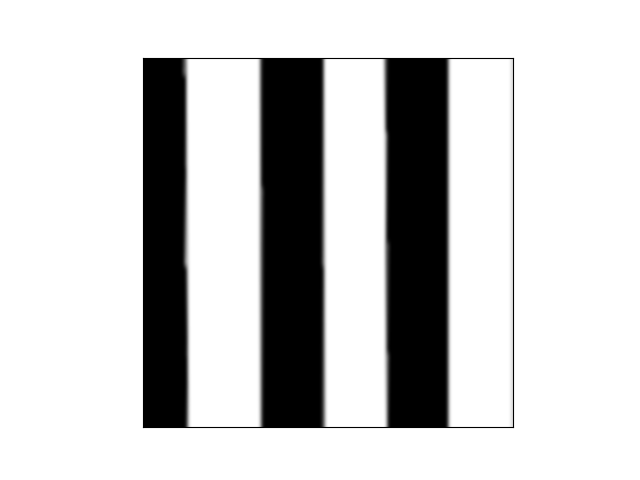
\includegraphics[width=\linewidth]{image/bipolar/97818.png}
      \caption{gamma=0.97818}
    \end{subfigure}%
    \begin{subfigure}{.5\textwidth}
      \centering
      
\includegraphics[width=\linewidth]{image/bipolar/99999.png}
      \caption{gamma=0.99999}
    \end{subfigure}
    \caption{典型情况下的双极系数}
    \end{figure}

\begin{figure}[h]
    \centering
    \begin{subfigure}{.5\textwidth}
        \centering
        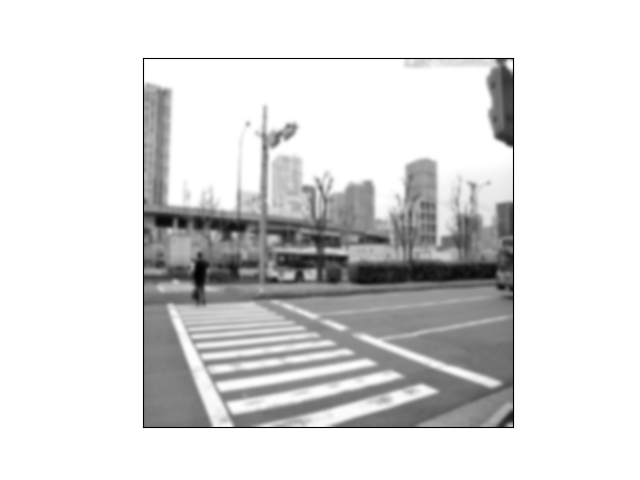
\includegraphics[width=\linewidth]{image/bipolar/64900.png}
        \caption{gamma=0.64900}
    \end{subfigure}%
    \begin{subfigure}{.5\textwidth}
        \centering
        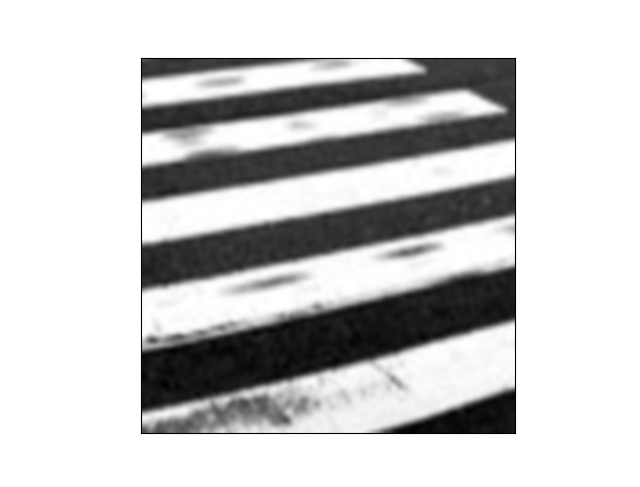
\includegraphics[width=\linewidth]{image/bipolar/72579.png}
        \caption{gamma=0.72579}
    \end{subfigure} \\
    \begin{subfigure}{.5\textwidth}
        \centering
        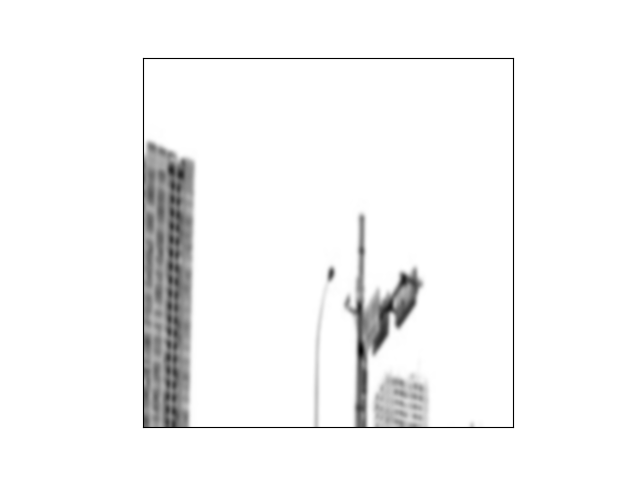
\includegraphics[width=\linewidth]{image/bipolar/29594.png}
        \caption{gamma=0.29594}
    \end{subfigure}%
    \begin{subfigure}{.5\textwidth}
        \centering
        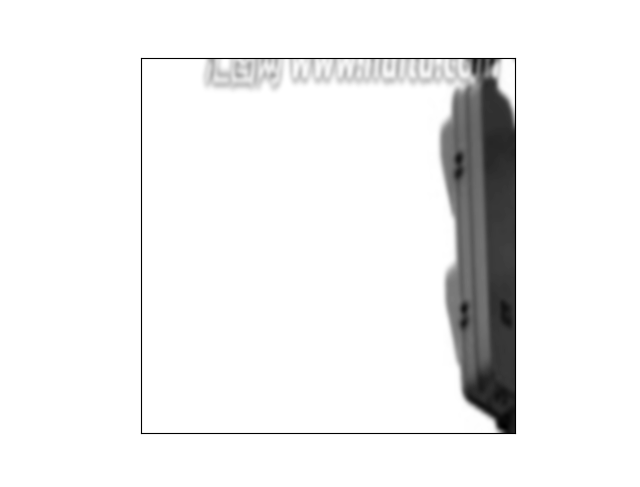
\includegraphics[width=\linewidth]{image/bipolar/90736.png}
        \caption{gamma=0.90736}
    \end{subfigure}
    \caption{现实照片中的双极系数}
    \end{figure}
\par
由以上图像示例说明,对于双极系数的推理是科学的,在现实的照片中也有体现,但仍有误识的情况。可以分析得到,双极系数法在现实情况中确实能反映出斑马线的特征,但方法特异性不高,它主要的门槛在于无法利用图片空间域的信息,比如邻接信息,聚类信息等等,单纯从灰度的统计信息出发难免有局限。
    
\section{Hough变换判据的研究}
我们从空间域特性出发,研究更加细致得斑马线判据。根据斑马线的特性,在ROI中只可能存在一组夹角不大的直线,而且直线之间呈现黑白相间的特点。因此我们可以首先对灰度化的ROI应用边缘检测算子,然后使用直线提取算法。在得到ROI中的一组直线之后,需要做一些特殊处理:
\begin{enumerate}
    \item 首先,要去除法向的干扰直线,做法是通过一个角度为$\frac{\pi}{4}$的滑动扇形来取出夹角在一个扇形以内的最多的直线,然后将其余直线全部删除。原因是即使是考虑如图4-1所示的平视视角也不会出现夹角大于$\frac{\pi}{4}$的斑马线边缘。
    \item 其次,要合并由于边缘检测产生的误差导致的接近重合的直线,如图4-2,在实现当中通过去除像素个数小于1000的区域来实现。
    \item 最后,这一组保留下来的直线,在ROI中不能相交,在实际操作中可以给干扰直线留出一点余量。
\end{enumerate}
\begin{figure}[h]
	\centering
	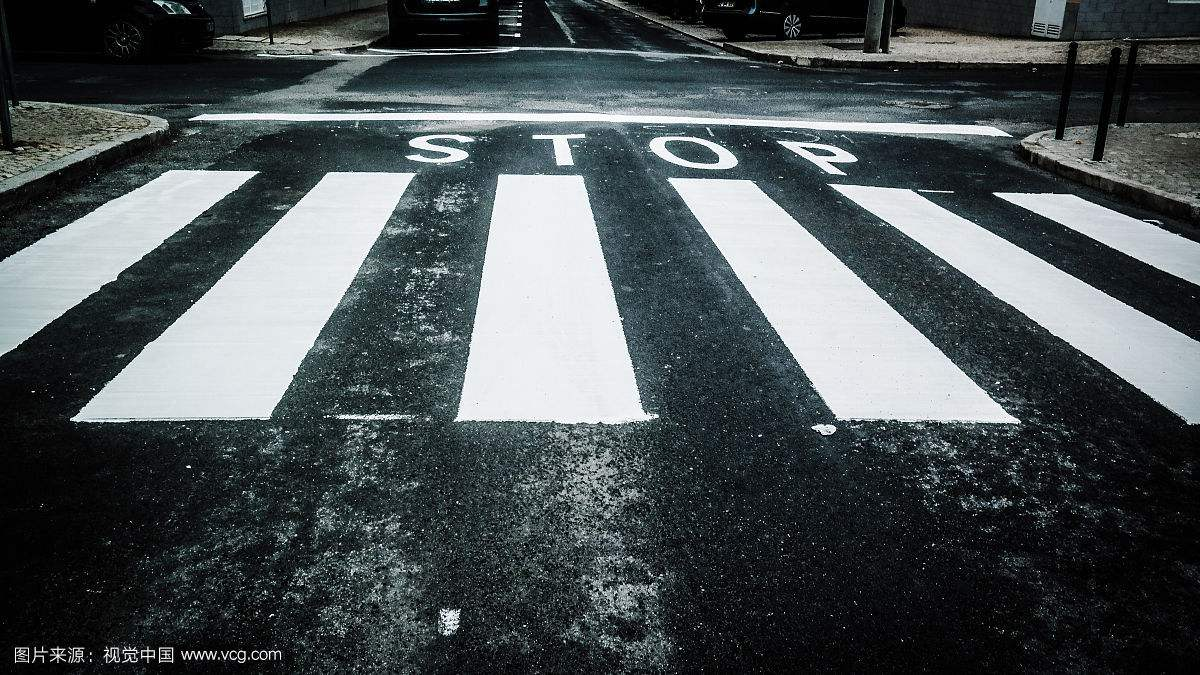
\includegraphics[width=0.5\textwidth]{image/sight.jpeg}
	\caption{平视斑马线}
\end{figure}
\begin{figure}[h]
	\centering
	
\includegraphics[width=0.5\textwidth]{image/line_merge_cut.png}
    \caption{删除重合直线}
\end{figure}
\par
当我们确定一组方向大致相同且在ROI内不相交的直线之后,我们实际上在二位平面上定义了序关系,我们按照法向遍历这些被直线分割的区域,按照二值化后白色占据绝对优势或者黑色占据绝对优势抑或两者都不是,确定一个形如BWBWBWXBXWBBW的字符串,然后通过字串匹配算法寻找BWBWBW和WBWBWB即可。
\begin{figure}[h]
	\centering
	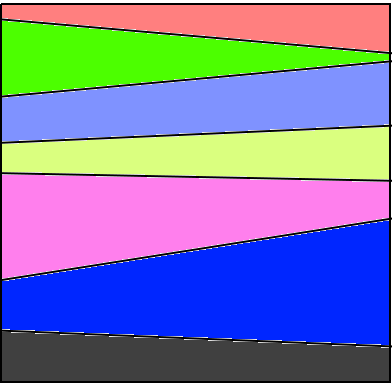
\includegraphics[width=0.5\textwidth]{image/order2.png}
	\caption{平面上的序关系}
\end{figure}

\section{纹理判据与支持向量机}
在实验结果中,Hough变换判据已经取得了不错的识别效果。为了进一步降低误识率提高准确率,我们可以把经过预处理的ROI视为一种纹理,进而使用纹理检测的技术判定斑马线。我们通过计算
\begin{align}
    dist=[1, 3, 5, 9] \\
    angle=[0, \frac{\pi}{4}, \frac{\pi}{2}, \frac{3 \times \pi}{4}, ]
\end{align}
共$16$个灰度共生矩阵,分别提取:熵、对比度、能量、反差分矩、相关性五个特征,构成一个$80$维的特征向量。通过学习算法来检测斑马线纹理。这次实验中我们采用支持向量机作为学习机。纹理判据在测试集上表现为在准确率下降不大的情况下,显著降低了误识率。\par
最终的判定依据为:
\begin{align}
    Predict=\left\{\begin{matrix}
        true & if \frac{\alpha}{4} + \frac{\beta}{4} + \frac{\gamma}{2} \geq \frac{1}{2} \\
        false & otherwise
        \end{matrix}\right.
\end{align}
$\alpha,\beta,\gamma$ 依次为4.1,4.2,4.3中判据的判定结果 
        \newclearpage
        %%
% 结论
% 结论是毕业论文的总结,是整篇论文的归宿,应精炼、准确、完整。结论应着重阐述自己的创造性成果及其在本研究领域中的意义、作用,还可进一步提出需要讨论的问题和建议。
% modifyer: 黄俊杰(huangjj27, 349373001dc@gmail.com)
% update date: 2017-04-13
%%

\chapter{试验结果}
在总图片数200张,其中包含斑马线的图片100张,不包含斑马线的图片100张。不包含斑马线的图片来自:无斑马线的街景、室内照片、建筑物、风景和一些随机图片。
\begin{table}[h] %voc table result
	\centering
		\begin{tabular}{*{4}{c}}
			\toprule
	 		Method & precision & recall \\
			\midrule
			双极系数 & 75.6 & 79 \\
		    Hough变换 & 88.3 & 80.6 \\
			支持向量机 & 86.4 & 93.7 \\
			加权判据 & 88 & 89.5 \\
			\bottomrule
		\end{tabular}
		\caption{实验对比表格}
\end{table}
\par
\begin{figure}[h]
    \centering
    \begin{subfigure}{.5\textwidth}
      \centering
      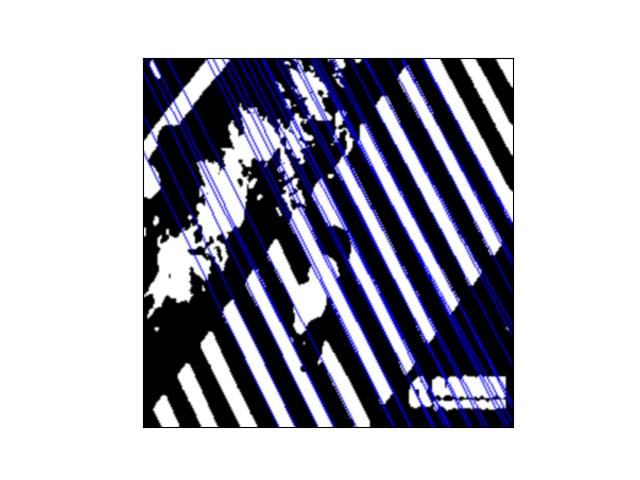
\includegraphics[width=\linewidth]{image/wrong1.png}
      \caption{颜色检测错误}
    \end{subfigure}%
    \begin{subfigure}{.5\textwidth}
      \centering
      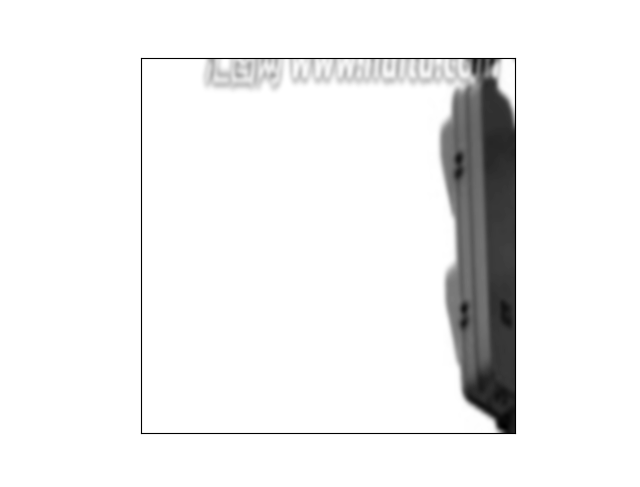
\includegraphics[width=\linewidth]{image/bipolar/90736.png}
      \caption{双极系数错误}
    \end{subfigure}
    \caption{典型情况错误分析}
\end{figure}
\par
已经观测到的错误原因如图5-1(a),Hough判据已经找出直线的情况下,由于斑马线恰好占据ROI的对角线,因此无法确认对应区域的颜色(黑色和白色几乎一样多)导致生成字符串中的一个B变为X。
另一种错误原因如图5-1(b),双极系数容易被黑白图片迷惑。


        \newclearpage
        %%
% 结论
% 结论是毕业论文的总结,是整篇论文的归宿,应精炼、准确、完整。结论应着重阐述自己的创造性成果及其在本研究领域中的意义、作用,还可进一步提出需要讨论的问题和建议。
% modifyer: 黄俊杰(huangjj27, 349373001dc@gmail.com)
% update date: 2017-04-13
%%
\chapter{总结与展望}
\section{工作总结}
本次工作由传统的双极系数法入手,探索双极系数法的优点和局限,顺藤摸瓜提出了空间域上的特征检测——Hough判据,与之前文章的不同之处在于,本文不单单考虑Hough变换后直线的个数和间隔,更考虑二值化后的颜色黑白间隔的特征进一步提高了识别的准确率。进一步创新地利用纹理检测的手段,从新的角度看待斑马线检测,并将该问题变成了一个可以应用机器学习的问题。
\section{研究展望}
首先一些如第五章中列出的已知错误,可以通过一些更加复杂和精确的技术来解决,这一部分有待填补。当抽象出纹理的特征向量后,可以有多种机器学习方法可以应用,例如决策树和神经网络,另外在训练数据和测试集方面还有增加的余地,对于三种判据优劣的具体分析还可以深入。斑马线检测,除了传统的特征检测与定位技术,是否可以看成通用的物体检测,这一点有待探究。本文的实验平台以python为主,包换OpenCV、skimage和sklearn,平均每张图片的处理需要4到5秒,这个速度如果用C++来重构代码,大约可以支撑8帧每秒的实时图片流,对于实时性要求基本满足,但提升空间还很大。
        \newclearpage
        % 结语

    % 附录部分
    \backmatter
        % 参考文献. 因不需要纳入章节目录, 故放入附录部分
        % 实际上参考文献是属于论文主体部分
        \makereferences

        %%
% 致谢
% 谢辞应以简短的文字对课题研究与论文撰写过程中曾直接给予帮助的人员(例如指导教师、答疑教师及其他人员)表示对自己的谢意,这不仅是一种礼貌,也是对他人劳动的尊重,是治学者应当遵循的学术规范。内容限一页。
% modifier: 黄俊杰
% update date: 2017-04-15
%%

\chapter{致谢}

\vskip 108pt
\begin{flushright}
	王天宇\makebox[1cm]{} \\
\today
\end{flushright}

    % 致谢
        \newclearpage
        % 附录
    \makeGrade      % 成绩评定记录表
\end{document}

